\documentclass[12pt, a4paper]{article}

% Typography (https://material.io/design/typography/the-type-system.html)

\newcommand{\headlineSix}[1]{
    {\LARGE #1}
}

\newcommand{\subtitleOne}[1]{
    {\Large #1}
}

\newcommand{\subtitleTwo}[1]{
    {\large #1}
}

% Iconography

\newcommand{\icon}[2][20pt]{
    \raisebox{-.25\height}{
        \includesvg[height=#1]{#2}
    }
}

% Table

\newcommand{\rowend}{
    \\[12pt]
}

\newcommand{\lineend}{
    \\[4pt]
}

\newcommand{\tabListItem}[1]{
    \textendash \hspace{4pt} #1
}

% Section

\newcommand{\sectionTitle}[2]{
    \raisebox{-.1\height}{
        \includesvg[height=20pt]{#2}
    }
    \headlineSix{\textbf{#1}}
}

\newcommand{\subsectionTitle}[2]{
    \subtitleOne{#1} \hfill #2
}

\newenvironment{sectionBody}{
    \vspace{-16pt}
    \begin{tabbing}
    \hspace{5mm} \= \\
}
{ 
    \end{tabbing}
    \vspace{-25pt}
}

\newenvironment{subsec}[2]{
    \subsectionTitle{#1}{#2}
    \begin{sectionBody}
}
{
    \end{sectionBody}
}

% Language
\usepackage[english]{babel}
\usepackage[utf8]{inputenc}
\usepackage{newunicodechar}

% Font
\usepackage[sfdefault]{roboto}

% Paging
\usepackage[a4paper, total={6in, 8in}, margin=1cm, showframe]{geometry}

% Image
\usepackage{graphicx}
\graphicspath{ {images/} }
\usepackage{svg}
\usepackage{float}

% Table
\usepackage{array}

% Metadata
\title{CV}
\author{Arcadii Rubailo}

% Global settings
\setlength{\intextsep}{0pt}
\setlength{\parindent}{0pt}

\setlength{\tabcolsep}{2pt}

% Content
\begin{document}
\begin{minipage}[t]{0.35\textwidth}
    \begin{figure}[H]
        \vspace*{-12pt}
        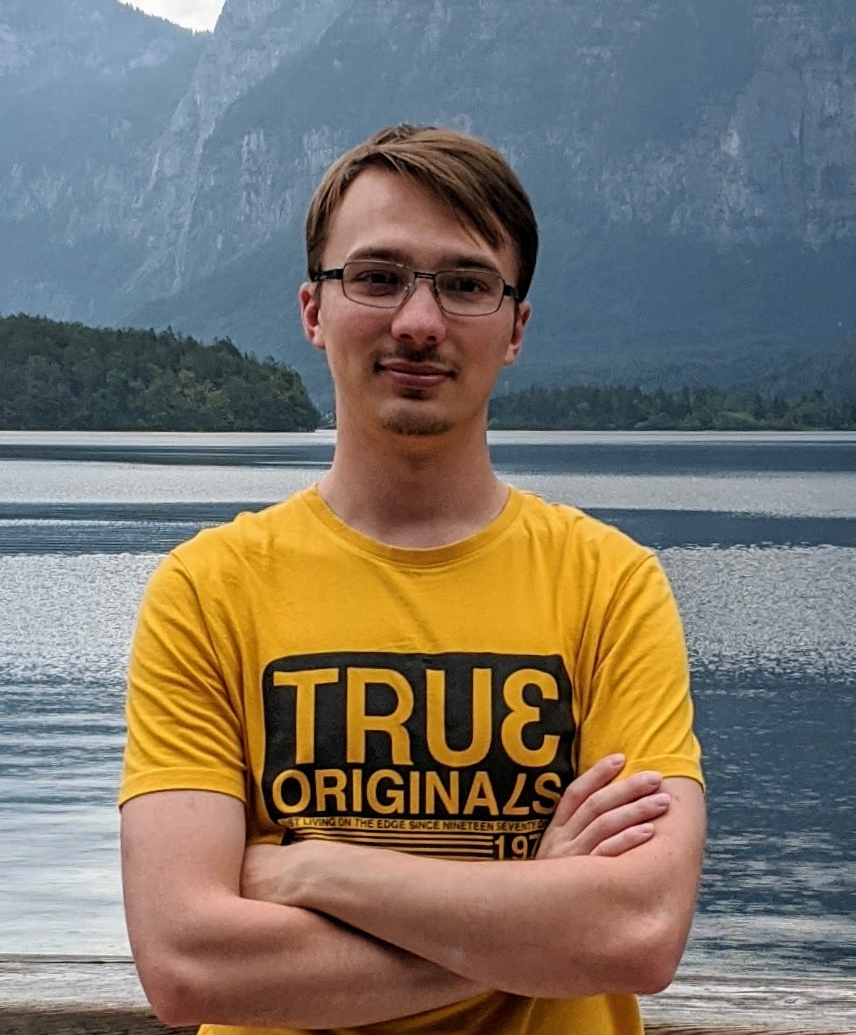
\includegraphics[width=\textwidth]{profile}
    \end{figure}
    
    \begin{center}
        \headlineSix{Arcadii Rubailo}
    \end{center}
    
    \begin{tabular}{ c l }
        \icon{icon_email}           &   rubailo.arcadii@gmail.com       \rowend
        \icon{icon_phone}           &   +420 775 087 503                \rowend
        \icon{icon_home}            &   Videnska 22d, Brno              \\
                                    &   Czech Republic                  \rowend
        \icon{icon_flag}            &   Moldova                         \rowend                        
        \icon[15pt]{icon_linkedin}  &   /arcadii-rubailo                \rowend
        \icon[18pt]{icon_github}    &   /elderanakain                   \rowend
        \icon{icon_list}            &   Programming languages:          \\
                                    &   Kotlin, Java.                   \rowend
                                    &   Development tools:              \\
                                    &   Android Studio,                 \\
                                    &   Zeplin, Jira, Figma.            \rowend
        \icon{icon_language}        &   Russian - Native                \\  
                                    &   English - C1                    \\  
                                    &   Romanian - B1                   \\  
                                    &   Czech - A1                      \rowend
    \end{tabular}
\end{minipage}
\hspace{15pt}
\begin{minipage}[t]{0.6\textwidth}
    \sectionTitle{Experience}{icon_work}
    
    \subsectionTitle{Kiwi.com}{07.2018 – Present}
    \begin{sectionBody}
        \> Kiwi.com Android app, booking main developer. \\
        \> Tech stack: Kotlin/Java, MVVM, Realm, ARCore, \\
        \> Dagger2/Koin, Databinding\&LiveData, Moshi/Gson, \\
        \> RxJava2/Flow, Jetpack Libraries, Retrofit2+OkHttp3. \\
    \end{sectionBody}
    
    \subsectionTitle{Ellation}{01.2017 – 08.2017}
    \begin{sectionBody}
        \> VRV and Crunchyroll Android apps development. \\
        \> Tech stack: Java/Kotlin, Retrofit2+OkHttp3, Chromecast, \\
        \> MVP, Fabric, Exoplayer, Firebase, Branch.io, \\
        \> Outbound.io, JUnit4, Mockito1. \\
    \end{sectionBody}
    
    \subsectionTitle{Yopeso}{08.2016 – 01.2017}
    \begin{sectionBody}
        \> limango Android app development. \\
        \> Tech stack: Java, Retrofit+OkHttp3, Firebase, RxJava, \\
        \> MVP, JUnit4+Mockito2, Dagger2, SQLite. \\
    \end{sectionBody}
    
    \subsectionTitle{Travod International}{10.2015 – 08.2016}
    \begin{sectionBody}
        \> Technical support, DTP and project management. \\
        \> Tech stack: Photoshop, InDesign, SDL Trados. \\
    \end{sectionBody}
     
    \subsectionTitle{Aursoft}{02.2015 – 12.2015}
    \begin{sectionBody}
        \> MyBebe Android app development. \\
        \> Tech stack: Java, Support Library, Volley, Picasso, SQLite. \\
    \end{sectionBody}
    
    \sectionTitle{Education}{icon_school}
    
    \subsectionTitle{Masaryk University}{2017 – 2019}
    \begin{sectionBody}
        \> MSc, Faculty of Informatics \\
        \> Service Science, Management and Engineering programme \\
    \end{sectionBody}
    
    \subsectionTitle{State University of Moldova}{2014 – 2017}
    \begin{sectionBody}
        \> BSc, Mathematics and Computer Science \\
        \> Computer science programme \\
    \end{sectionBody}
\end{minipage}
\end{document}
